% Example LaTeX document for GP111 - note % sign indicates a comment


\documentclass{article}
\usepackage{graphicx}
\usepackage{color}
\graphicspath{ {./images/} }

\definecolor{dkgreen}{rgb}{0,0.6,0}
\definecolor{gray}{rgb}{0.5,0.5,0.5}
\definecolor{mauve}{rgb}{0.58,0,0.82}

\usepackage{listings}

\lstset{frame=tb,
  language=Python,
  aboveskip=3mm,
  belowskip=3mm,
  showstringspaces=false,
  columns=flexible,
  basicstyle={\small\ttfamily},
  numbers=none,
  numberstyle=\tiny\color{gray},
  keywordstyle=\color{blue},
  commentstyle=\color{dkgreen},
  stringstyle=\color{mauve},
  breaklines=true,
  breakatwhitespace=true,
  tabsize=3
}
\graphicspath{ {./images/} }
% Default margins are too wide all the way around. I reset them here
\setlength{\topmargin}{-.5in}
\setlength{\textheight}{9in}
\setlength{\oddsidemargin}{.125in}
\setlength{\textwidth}{6.25in}
\begin{document}
\title{Beer Game Part-1}
\author{Sam Reifenstein, Koji Sunami, Jack McKee}
\renewcommand{\today}{April 26, 2019}
\maketitle
\section*{Code}
Here is our code, written in SageMath:
\begin{lstlisting}
import collections

#parameters
Params = collections.namedtuple('Params', ['alpha', 'beta', 'theta', 'Q', 'RIO']);

#initial values of variables
Point = collections.namedtuple('Point', ['FI', 'FB', 'FPD2', 'FPD1', 'FPR', 'FOS', 'FIO', 'FED', 'FSL', 'RI', 'RB', 'RIS', 'RIO', 'RED', 'ROP', 'RSL'])
init = Point(1,1,1,1,1,1,1,1,1,1,1,1,1,1,1,1)

#handy iterator class

class FunctionIter:
    x = 0
    f = lambda x: x
    step = 1
    n = 0
    m = 1
    def __init__(self,init,func,n,step):
        self.x = init
        self.f = func
        self.m = n
        self.step = step
    def __iter__(self):
        return self
    def next(self):
        ret = self.x
        for i in range(self.step):
            self.x = self.f(self.x)
        self.n = self.n + 1
        if self.n > self.m:
            raise StopIteration
        return ret


my_l = [];
def iterate(N, params):
	
	def do_beer_game(x):
		_FI = max(0,x.FI + x.FPD2 - x.FB - x.FIO)
		_FB = max(0,x.FB + x.FIO - x.FI - x.FPD2)
		_FED = params.theta*x.FIO + (1-params.theta)*x.FED
		_FSL = x.FPR + x.FPD1 #FSL_n = FPD1_n + FPD2_n = FPR_n-1 + FPD1_n-1
		_FOS = min(x.FI + x.FPD2, x.FB + x.FIO)
		_RI = max(0,x.RI + x.RIS - x.RB - params.RIO)
		_RB = max(0,x.RB + params.RIO - x.RI - x.RIS)
		_RED = params.theta*x.RIO + (1-params.theta)*x.RED
		_RSL = x.FOS + x.ROP + _FB + _FOS #RSL_n = RIS_n + FIO_n + FB_n + FOS_n = FOS_n-1 + ROP_n-1 + FB_n + FOS_n
		return Point(FI = _FI,
					 FB = _FB,
					 FPD2 = x.FPD1,
					 FPD1 = x.FPR,
					 FPR = max(0,_FED + params.alpha*(params.Q - _FI + _FB - params.beta*_FSL)),
					 FOS = _FOS,
					 FIO = x.ROP,
					 FED = _FED,
					 FSL = _FSL,
					 RI = _RI,
					 RB = _RB,
					 RIS = x.FOS,
					 RIO = params.RIO,
					 RED = _RED,
					 ROP = max(0,_RED + params.alpha*(params.Q - _RI + _RB - params.beta*_RSL)),
					 RSL = _RSL)
	global my_l
	my_l = list(FunctionIter(init,do_beer_game,N,1))
	
FI_l = lambda x: my_l[floor(x)+1].FI*(x - floor(x)) + my_l[floor(x)].FI*(1-x+floor(x))
FB_l = lambda x: my_l[floor(x)+1].FB*(x - floor(x)) + my_l[floor(x)].FB*(1-x+floor(x))
FPD1_l = lambda x: my_l[floor(x)+1].FPD1*(x - floor(x)) + my_l[floor(x)].FPD1*(1-x+floor(x))
FPD2_l = lambda x: my_l[floor(x)+1].FPD2*(x - floor(x)) + my_l[floor(x)].FPD2*(1-x+floor(x))
FPR_l = lambda x: my_l[floor(x)+1].FPR*(x - floor(x)) + my_l[floor(x)].FPR*(1-x+floor(x))
FOS_l = lambda x: my_l[floor(x)+1].FOS*(x - floor(x)) + my_l[floor(x)].FOS*(1-x+floor(x))
FIO_l = lambda x: my_l[floor(x)+1].FIO*(x - floor(x)) + my_l[floor(x)].FIO*(1-x+floor(x))
FED_l = lambda x: my_l[floor(x)+1].FED*(x - floor(x)) + my_l[floor(x)].FED*(1-x+floor(x))
FSL_l = lambda x: my_l[floor(x)+1].FSL*(x - floor(x)) + my_l[floor(x)].FSL*(1-x+floor(x))
RI_l = lambda x: my_l[floor(x)+1].RI*(x - floor(x)) + my_l[floor(x)].RI*(1-x+floor(x))
RB_l = lambda x: my_l[floor(x)+1].RB*(x - floor(x)) + my_l[floor(x)].RB*(1-x+floor(x))
RIS_l = lambda x: my_l[floor(x)+1].RIS*(x - floor(x)) + my_l[floor(x)].RIS*(1-x+floor(x))
RED_l = lambda x: my_l[floor(x)+1].RED*(x - floor(x)) + my_l[floor(x)].RED*(1-x+floor(x))
ROP_l = lambda x: my_l[floor(x)+1].ROP*(x - floor(x)) + my_l[floor(x)].ROP*(1-x+floor(x))
RSL_l = lambda x: my_l[floor(x)+1].RSL*(x - floor(x)) + my_l[floor(x)].RSL*(1-x+floor(x))
# plot all the different lists in different colors
def plotTrajectories(plot_begin, plot_end): 
	show(plot([FI_l,
			   FB_l,
			   FPD1_l,
			   FPD2_l,
			   FPR_l,
			   FOS_l,
			   FIO_l,
			   FED_l,
			   FSL_l,
			   RI_l,
			   RB_l,
			   RIS_l,
			   RED_l,
			   ROP_l,
			   RSL_l],
			   color = 'automatic',
			   legend_label = ["FI",
							   "FB",
							   "FPD1",
							   "FPD2",
							   "FPR",
							   "FOS",
							   "FIO",
							   "FED",
							   "FSL",
							   "RI",
							   "RB",
							   "RIS",
							   "RED",
							   "ROP",
							   "RSL"],
			   xmin = plot_begin,
			   xmax = plot_end))
def plotTwoComponents(var1, var2, plot_begin, plot_end):
	
	show(list_plot((map(lambda x : (getattr(x, var1), getattr(x, var2)), my_l)[plot_begin: plot_end]), plotjoined = True), axes_labels = ('$'+var1+'$', '$'+var2+'$'))
import IPython
IPython.embed()

\end{lstlisting}

\section*{Example 1}
These parameters appear to give a periodic attractor with period around 15.
\linebreak
Code:
\begin{lstlisting}
#set parameters:
params = Params(alpha = 1.0,
				beta = 0.5,
				theta = 0.5,
				Q = 0.5,
				RIO = 5 #for now, demand is constant
			)


#iterate the map to 1000 steps
iterate(1000, params)

#plot parameters
plot_begin = 0
plot_end = 100

#plot the trajectory of each variable 
plotTrajectories(plot_begin, plot_end)

#plot the factory's inventory against the factory's incoming orders
plotTwoComponents("FI", "FIO", plot_begin, plot_end)
\end{lstlisting}
Output:
\linebreak
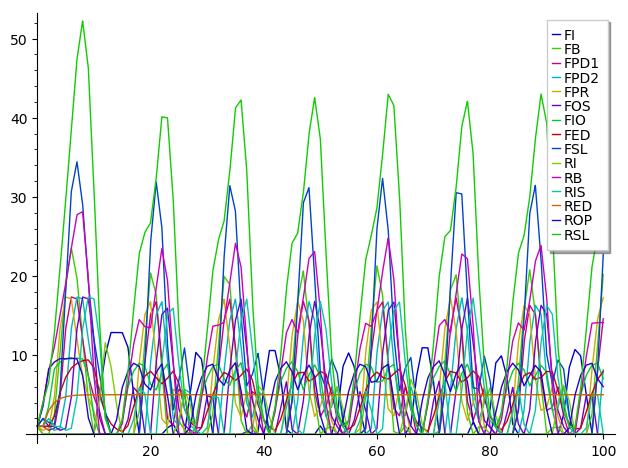
\includegraphics[scale=1.0]{example1_1.png}
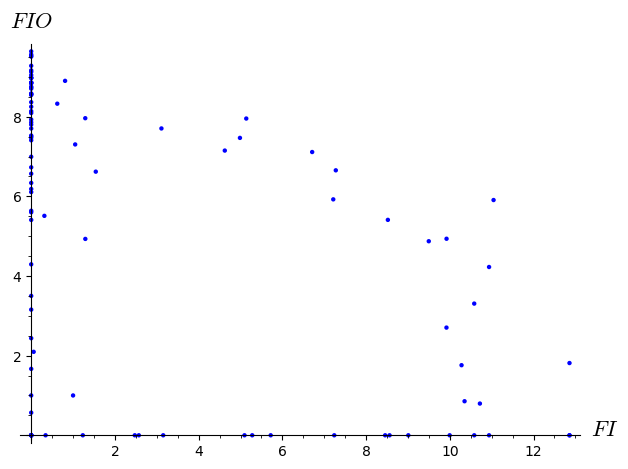
\includegraphics[scale=1.0]{example1_2.png}

\section*{Example 2}
These parameters seem to result in chaos. I gave a much larger time scale to demonstrate that the trajectory doesn't seem to settle down in a pattern.
\linebreak
Code:
\begin{lstlisting}
#set parameters:
params = Params(alpha = 1.6,
				beta = 0.2,
				theta = 0.6,
				Q = 0.1,
				RIO = 5 #for now, demand is constant
			)


#iterate the map to 5000 steps
iterate(5000, params)

#plot parameters
plot_begin = 0
plot_end = 2000

#plot the trajectory of each variable 
plotTrajectories(plot_begin, plot_end)

#plot the factory's inventory against the factory's incoming orders
plotTwoComponents("FI", "RI", plot_begin, plot_end)
\end{lstlisting}
Output:
\linebreak
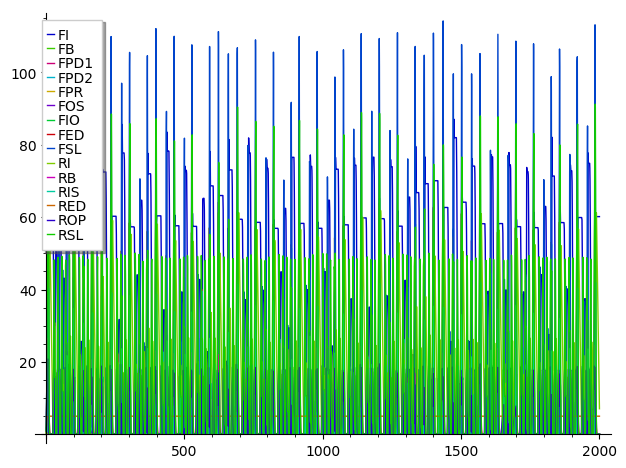
\includegraphics[scale=1.0]{example2_1.png}
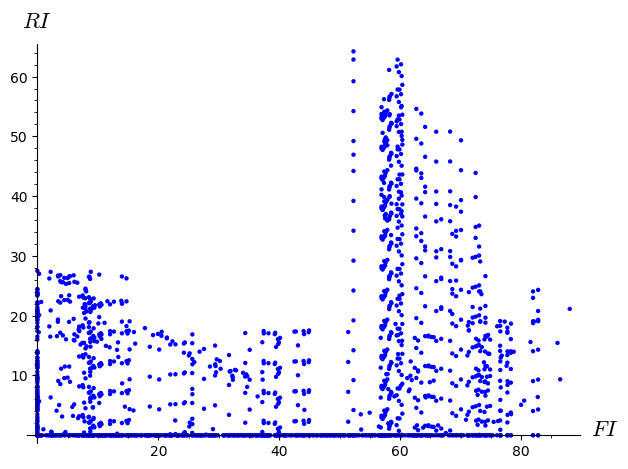
\includegraphics[scale=1.0]{example2_2.png}


\end{document}
